\chapter{Database \& Data Center Security}

\section{Introduzione}

Negli ultimi anni il modello di Database Relazionale è diventato molto popolare ed ampiamente utilizzato da
privati e aziende.
Per molte organizzazioni, è importante essere in grado di
fornire a clienti, partner e dipendenti l'accesso alle informazioni da loro memorizzate. Ma tali
informazioni possono essere prese di mira da minacce interne ed esterne, possono essere utilizzate
impropriamente o modifiche da entità non autorizzate. Di conseguenza, la sicurezza
specificamente adattata ai database è una componente sempre più importante di una strategia generale per la protezione dei dati.

Di seguito andremo ad elencare le principali ragioni per cui la sicurezza dei database non ha tenuto il passo con
l'aumento della dipendenza dai database:

\begin{enumerate}
      \item C'è un drammatico squilibrio tra la complessità dei moderni
            database (DBMS) e le tecniche di sicurezza usate per proteggere questi
            sistemi critici. Un DBMS è un software molto complesso e di grandi
            dimensioni, che fornisce molte opzioni, che devono essere tutte ben
            comprese e poi protette per evitare violazioni dei dati.
      \item I database hanno un sofisticato protocollo di interazione chiamato
            \textit{Structured Query Language} (\textbf{SQL}),
            che è molto complesso e potente, quindi deve essere appreso pienamente
            prima di poter essere utilizzato.
      \item La mancanza di personale specializzato. L'azienda media non ha
            personale addetto alla gestione della sicurezza di database.
            Generalmente hanno uno staff per la sola amministrazione del DB che
            non è sufficientemente formato per gestirne anche la sicurezza.
      \item La maggior parte degli ambienti aziendali consiste in una miscela
            eterogenea di piattaforme di database, piattaforme aziendali e OS,
            quindi non avere un solo db o un solo tipo di sistema operativo
            rappresenta una problematica che crea un'ulteriore complessità per il
            personale.
      \item La crescente dipendenza dalla tecnologia cloud per ospitare parte o
            tutto il database aziendale risulta essere un'ulteriore sfida in quanto
            aggiunge ulteriori oneri per il
            personale di sicurezza.
\end{enumerate}

Possiamo definire quindi un \textbf{Database} come una raccolta strutturata di
dati immagazzinati e messi in relazione tra di loro per essere utilizzati da una
o più applicazioni; organizzati in tabelle che possono essere manipolate tramite
un apposito linguaggio chiamato Data Definition Language (\textbf{DDL}); recuperati
tramite un apposito linguaggio di query standardizzato (\textbf{SQL}) e gestiti
da un apposito software chiamato \textbf{Database Management System}.\\

Il principale vantaggio dei Database, oltre alla possibilità di organizzare e
recuperare informazioni in pochissimo tempo, è quella di poter limitare l'accesso
e la visibilità solo a singole parti di un determinato file. Nei classici sistemi
operativi questo non risulta possibile dato che si può solo specificare se un
utente può o no accedere ad un file ma non limitarne la visibilità solo ad una
sua parte.

\section{SQL Injection Attack}

Gli attacchi di tipo SQL Injection sono una delle minacce alla sicurezza diffuse
e pericolose. Questo attacco si basa sull'invio di dati contenenti una
parte di query malevola per l'estrazione, modifica o cancellazione di tutti i
dati presenti all'interno di un database fruibile tramite un'applicazione web.

\begin{figure}[H]
      \centering
      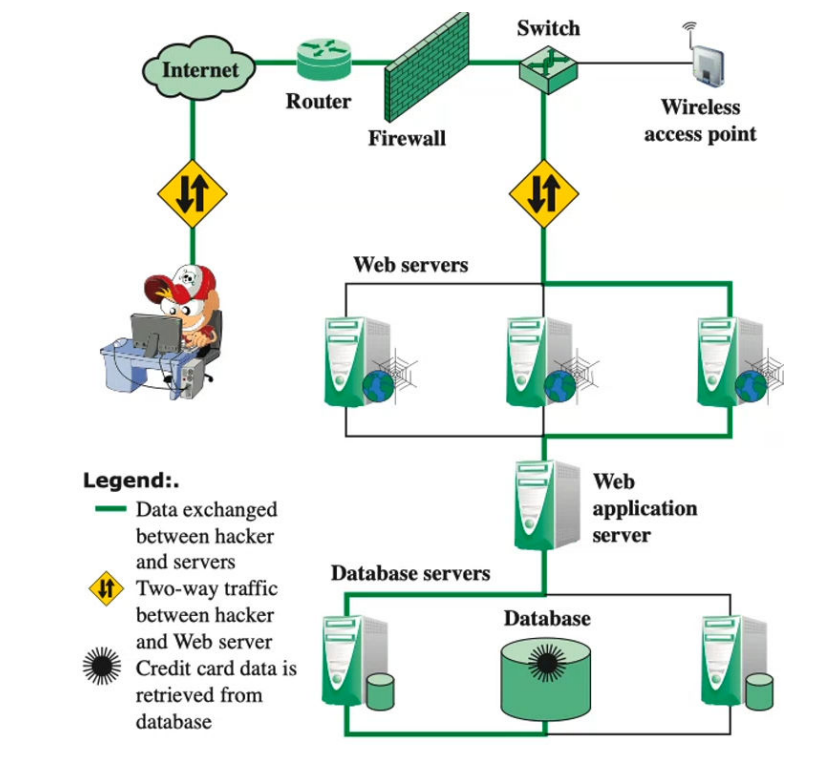
\includegraphics[width=10cm, keepaspectratio]{capitoli/sql_security/imgs/sql1.png}
      \caption{Esempio di un tipico attacco SQL Injection.}
\end{figure}

Questo attacco funziona tipicamente terminando prematuramente una stringa di
testo, generalmente con un commento \verb|--|, e aggiungendo un nuovo comando
che verrà eseguito dal database ed impedirà l'esecuzione del resto della query.\\

Possiamo caratterizzare gli attacchi SQL Injection in termini di via d'attacco e
tipo di attacco.

\subsection{Attack Avenues}

\begin{figure}[H]
      \centering
      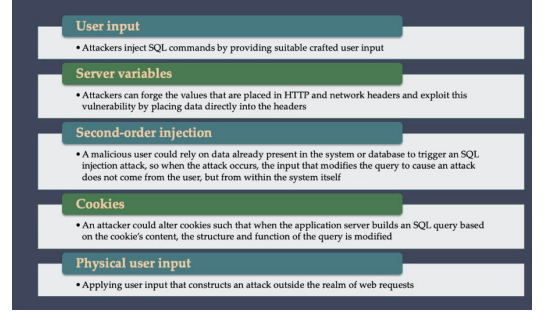
\includegraphics[width=10cm, keepaspectratio]{capitoli/sql_security/imgs/sql3.png}
\end{figure}

Le principali vie d'attacco sono le seguenti:

\paragraph{Input dell'utente:}
l'aggressore fornisce al database un input opportunamente modificato per
forzare l'esecuzione di una query malevola.

\paragraph{Variabili server:}
Le variabili del server sono un insieme di variabili che contengono intestazioni
HTTP, intestazioni del protocollo di rete e variabili ambientali. Le
applicazioni web usano queste variabili del server in una varietà di modi, come
la registrazione di statistiche e informazioni di utilizzo per identificare le
tendenze di un utente. Se queste variabili sono registrate in un database senza
sanificazione, questo potrebbe creare una vulnerabilità di SQL injection in
quanto è possibile modificarle ed inserirci codice arbitrario.

\paragraph{Second Order Injection:}
Un attaccante può sfruttare dati già presenti nel sistema o nel database per
attivare un attacco SQL Injection cosicché quando avviene effettivamente
l'attacco la query malevola non proviene dall'utente ma direttamente dal sistema
stesso.

\paragraph{Cookie:}
Di solito vengono utilizzati anche i cookie per creare in modo automatico query
per salvare dati o manipolarli. Un attaccante può modificare il contenuto di un
cookie per andare a forzare l'esecuzione di una query maligna all'interno di un
database.

\paragraph{Input fisico dell'utente:}
Gli attacchi SQL Injection possono anche avvenire all'esterno di una richiesta
web: prendiamo in considerazione un sistema che in automatico scannerizza e
archivia documenti tramite l'ausilio di modelli di machine learning, questo può
essere attaccato scrivendo fisicamente una query malvagia all'interno del
documento da acquisire.


\subsection{Attack Types}

I tipi di attacco possono essere raggruppati in tre categorie principali:
\textbf{In-band}, \textbf{Inferential}, \textbf{Out of Band}.

\paragraph{In-Band.}
Un attacco in banda utilizza lo stesso canale di comunicazione per iniettare
codice SQL e recuperare i risultati. I dati recuperati sono presentati
direttamente nella pagina web dell'applicazione. I tipi di attacco In-Band
includono i seguenti:

\begin{itemize}
      \item \textbf{Tautologia}: Questa forma di attacco inietta codice in una o
            più dichiarazioni condizionali in modo che valutino sempre vero.
      \item \textbf{Commento di fine riga}: Dopo aver iniettato codice in un
            particolare campo, il codice legittimo che segue viene annullato
            attraverso l'uso di commenti di fine riga. Un esempio potrebbe
            essere quello di aggiungere "\verb|--|" dopo gli input in modo che
            le query rimanenti non siano trattate come codice eseguibile, ma come
            commenti.
      \item \textbf{Query piggybacked}: L'attaccante riesce ad aggiunge ed
            eseguire ulteriori query oltre a quella originale. Questa
            tecnica si basa su configurazioni del server che permettono diverse
            query all'interno di una singola stringa di codice.
\end{itemize}

\paragraph{Inferential.}
Sono attacchi che non fanno trasferimento dei dati, quindi sono attacchi su
confidenzialità e non integrità. L'attaccante è in
grado di ricostruire le informazioni e risalire a specifiche segrete del database
inviando particolari richieste
e osservando il comportamento risultante del server.
Le principali metodologie di attacco sono:
\begin{itemize}
      \item \textbf{Query illegali/logicamente scorrette:} La vulnerabilità
            sfruttata da questo metodo è che la pagina di errore
            predefinita restituita dai server delle applicazioni è
            spesso eccessivamente descrittiva. Infatti, il semplice
            fatto che viene generato un messaggio di errore può
            spesso rivelare parametri vulnerabili per un
            attaccante.

      \item \textbf{Blind SQL Injection:} Permette agli attaccanti di dedurre i
            dati presenti in un sistema di database anche quando il sistema è
            sufficientemente sicuro da non mostrare alcuna informazione errata
            all'attaccante.
\end{itemize}

\paragraph*{Out-of-band.}
Sono degli attacchi in cui l'input dell'attacco avviene per un canale e l'output
per un altro canale. In un attacco fuori banda, i dati vengono recuperati
utilizzando un canale diverso, ad esempio una e-mail con i risultati della query
viene generata e inviata all'attaccante. Questo può essere utilizzato quando ci
sono limitazioni sul recupero delle informazioni, ma la connettività in uscita
dal server del database non presenta importanti restrizioni.\footnote{Questo
      concetto è finemente espresso con la seguente parola: \textit{lassista}
      \emoji{teacher-light-skin-tone}.}

\section{SQL Injection Mitigation}

Poiché gli attacchi SQL Injection sono così diffusi, dannosi e variegati sia per
via dell'attacco che per tipo, una singola contromisura non è sufficiente.
Piuttosto un insieme integrato di tecniche è necessario. Le contromisure possono
essere classificate in tre tipi: \textit{Defensive Coding}, \textit{Detection},
e \textit{Run-time Prevention}.

\begin{figure}[H]
      \centering
      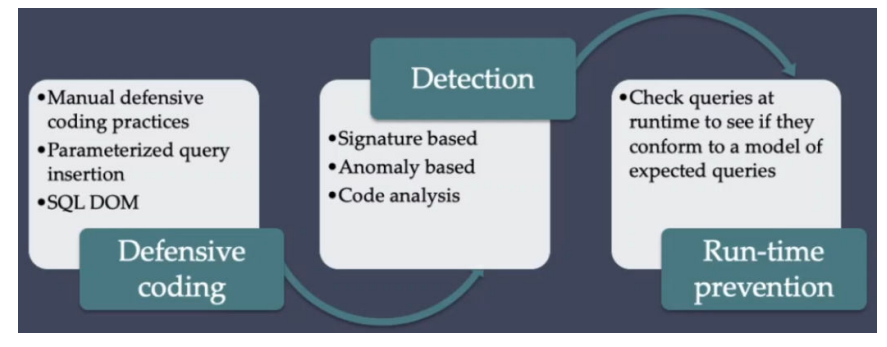
\includegraphics[width=12cm, keepaspectratio]{capitoli/sql_security/imgs/sql2.png}
\end{figure}

\paragraph{Defensive Coding:}
\begin{itemize}
      \item \textbf{Pratiche manuali di codifica difensiva}: Una vulnerabilità
            comune sfruttata da SQL Injection è l'insufficiente convalida
            dell'input. La soluzione semplice per eliminare queste vulnerabilità
            è applicare adeguate pratiche di codifica difensiva. Un esempio è il
            controllo del tipo di input, per verificare che gli input che si
            suppone siano essere numerici non contengano caratteri diversi dalle
            cifre. Questo tipo di tecnica può evitare attacchi basati sulla
            forzatura di errori nel sistema di gestione del database.Un altro
            tipo di pratica di codifica è quella che esegue il pattern matching
            per cercare di distinguere l'input normale da quello anormale.
      \item \textbf{Inserimento di query parametrizzate}: Questo approccio cerca
            di prevenire l'SQL Injection permettendo allo sviluppatore
            dell'applicazione di specificare più accuratamente la struttura di
            una query SQL, e passare i parametri di valore ad essa separatamente
            in modo che qualsiasi input dell'utente non possa
            modificare la struttura della query.
      \item \textbf{SQL DOM}: è un insieme di classi che permette la
            validazione automatica del tipo di dati, la validazione e l'escape.
            Questo approccio usa l'incapsulamento delle query di database per
            fornire un modo sicuro e affidabile per accedere ai database. Questo
            cambia il processo di costruzione delle query da un processo non
            regolamentato che usa la concatenazione di stringhe ad uno
            sistematico che utilizza un'API controllata.
\end{itemize}

\paragraph{Detection:}
\begin{itemize}
      \item \textbf{Signature based}: Questa tecnica tenta di rilevare specifici
            pattern di attacco in quanto ogni tipologia di attacco presenta
            un'esecuzione simile. Similmente agli antivirus questa contromisura
            deve essere costantemente aggiornata in quanto cambiare anche di pochissimo
            il pattern di attacco potrebbe renderlo non rilevabile.
      \item \textbf{Anomaly Based}: Questo approccio tenta di definire il
            comportamento normale e poi rilevare i modelli di comportamento al
            di fuori della gamma normale. C'è una fase di
            addestramento, in cui il sistema impara la gamma di comportamenti
            normali, seguita dalla fase di rilevamento vera e propria.
      \item \textbf{Code Analysis}: Le tecniche di analisi del
            codice coinvolgono l'uso di una suite di test per rilevare le
            vulnerabilità. La suite di test è progettata per generare una
            vasta gamma di attacchi e valutare la risposta del sistema.
\end{itemize}

\paragraph{Run-time Prevention:}
Queste tecniche controllano le query in fase di esecuzione per vedere se risultano
conformi ad un modello di query attese. Sono disponibili vari strumenti
automatizzati per questo scopo.
%% continuare fino a pagina 138